\documentclass{article}
\usepackage{graphicx} % Required for inserting images

\usepackage[top=0.5in]{geometry}
\usepackage{amsmath}
\usepackage{amsfonts}
\usepackage{listings}
\usepackage{setspace}
\usepackage{titlesec}
\usepackage{subcaption}
\usepackage{float}
\usepackage{appendix}
\usepackage{url}

\title{TASP: Solving TSP using Simulated Annealing}
\author{
    Artur Topal \texttt{(s5942128)} \\
    Juan Diego Sersen Valdeiglesias \texttt{(s5996848)}
}
\date{\today}

\begin{document}
\maketitle

\section{Problem Description}

The Traveling Salesman Problem (TSP) is a well-known problem in computing science and combinatorial optimization with numerous real-life applications in areas such as logistics, manufacturing, and network design. TSP can be summarized as a graph problem where one has to find the shortest possible route that visits each vertex exactly once and returns to the starting vertex.

TSP is known to be an NP problem where the brute force approach, which checks all possible routes, has a time complexity of \( O(n!) \), making it impractical for large inputs. Consequently, non-deterministic algorithms have been developed to find near-optimal solutions in a reasonable amount of time.
This project implements \textbf{Simulated Annealing}, a probabilistic optimization method inspired by the physical process, to find a locally optimal solution to TSP.
\\
\\
\textbf{Input.} All parameters to the program can be tweaked via command-line options and the graph can be input randomly or from the standard input. In this report, we use the following run command\footnote{ATT48 is a dataset with 48 cities from USA.}:  \\
tasp --temp=5000 -m40 -Mstd -Asolve $<$ att48.txt \\
where att48.txt is: \\
48          \\
6734 1453   \\
2233   10   \\
5530 1424   \\
 401  841   \\
3082 1644   \\
7608 4458   \\
7573 3716   \\
7265 1268   \\
6898 1885   \\
1112 2049   \\
5468 2606   \\
5989 2873   \\
4706 2674   \\
4612 2035   \\
6347 2683   \\
6107  669   \\
7611 5184   \\
7462 3590   \\
7732 4723   \\
5900 3561   \\
4483 3369   \\
6101 1110   \\
5199 2182   \\
1633 2809   \\
4307 2322   \\
 675 1006   \\
7555 4819   \\
7541 3981   \\
3177  756   \\
7352 4506   \\
7545 2801   \\
3245 3305   \\
6426 3173   \\
4608 1198   \\
  23 2216   \\
7248 3779   \\
7762 4595   \\
7392 2244   \\
3484 2829   \\
6271 2135   \\
4985  140   \\
1916 1569   \\
7280 4899   \\
7509 3239   \\
  10 2676   \\
6807 2993   \\
5185 3258   \\
3023 1942   \\

\textbf{Output.} Output must be the cost of the shortest close path that visits each city once. The globally optimal path is $33523$. The program gives the number $34978$ which is a very good result.  

\section{Problem Analysis}
\label{analysis}

Simulated annealing is inspired by the process of slowly cooling a heated metal to make it stronger, rather than cooling it rapidly. When cooling is gradual, atoms have an opportunity to move away from suboptimal positions, local minima in energy, and settle into more stable configurations. This idea is applied by allowing for occasional acceptance of worse solutions to escape local minima.

Let \( C_0 \) be the initial configuration of \( n \) cities, and let its energy \( E_0 \) represent the total path cost. We also choose an initial temperature \( T_0 \), which controls the probability of accepting worse routes. A new candidate configuration \( C_{\text{temp}} \) is generated with energy \( E_{\text{temp}} \). The next configuration \( C_1 \) is chosen as follows:

\begin{itemize}
    \item If \( E_{\text{temp}} < E_0 \): the new configuration \( C_{\text{temp}} \) is always accepted.
    \item If \( E_{\text{temp}} \ge E_0 \): the new configuration is accepted with probability
    \[
    P = e^{\frac{E_0 - E_{\text{temp}}}{kT}}
    \]
    where \( k \) is a constant. Otherwise, \( C_1 = C_0 \).
\end{itemize}

This probability function means that worse solutions are less likely to be accepted, especially as \( T \) decreases. In real annealing, \( k \) is Boltzmann’s constant, but since this process is simulated, we can simply set \( k = 1 \) and adjust the starting temperature \( T_0 \) to achieve the best performance.

\section{Design}

\subsection{System Overview}

The program consists of several self-contained modules such as:

\begin{itemize}
    \item \textbf{Main module:} Handles program initialization, argument parsing, and coordination of all other modules.
    \item \textbf{Graph module:} Abstraction of the graph including creation, distance matrix, and displaying.
    \item \textbf{Path module:} Functions that operate on paths. Each path is represented as an array of indices of vertices in a graph. Among others, the path module contains random permutation generators, cost-computing functions, and helper functions. 
    \item \textbf{Solver module:} Implements the Simulated Annealing algorithm.
\end{itemize}

On the more technical side, the program uses the notion of public and internal headers. The former ones are the headers that provide the interface (functions, data structures, etc.) for the use by other modules. Internal headers declare all the functions and data structures that can be hidden from other modules or the user. For instance, solve.h has one public function (sim\_annealing) and one private function (update) used internally. Each function has its own translation unit which allows for easier navigation.

Lastly, each internal header is compiled into a PCH\footnote{precompiled header} which drastically decreases the compilation time.

\subsection{More on the Data Structure Design}

Each city is represented by integer coordinates $(x_i, y_i)$ in the range that can be defined by command-line arguments, and each city has an ID equal to its index in the vertices array of the graph. The distance matrix of the graph uses Euclidean distance:

\[
d(i, j) = \sqrt{(x_i - x_j)^2 + (y_i - y_j)^2}.
\]

The distances are precomputed and stored in a two-dimensional matrix before the annealing process begins.  

A path is represented as a permutation of city indices \([0, 1, 2, ..., n-1]\).  
The cost (energy) of a path is calculated as the sum of distances between consecutive cities, returning to the starting city.

\subsection{Algorithm Design}

The Simulated Annealing algorithm is implemented as an iterative procedure that improves the solution by exploring and accepting new routes according to the function described section \ref{analysis}. The pseudocode for the algorithm is:

\begin{tabbing}
xxx \= xxx \= xxx \= xxx \= \kill
\textbf{algorithm} Annealing($G(V, D)$, $T$, $\bar{T}$, $m$, $\bar{I}$, $f: \mathbb{R} \rightarrow \mathbb{R}$) \\ 
\textit{input}:                                         \\
\> 1) graph $G$ with cities $V$ and distance matrix $D$ \\ 
\> 2) start and desired temperature $T, \bar{T}$        \\
\> 3) per-temperature number of iterations $m$          \\
\> 4) desired no-improvement number $\bar{I}$           \\
\> 5) the function $f$ that is used to decrease the temperature. \\
\textit{output}: \\
\> shortest path $\vec{b}$ that visits each vertex of $G$ once. \\
\\ 
\> Initialize $\vec{b}$ to starting path. \\
\> Initialize $\vec{c}$ to starting path. (candidate) \\
\> \textbf{let} I = 0 (current number of iterations without improvement) \\
\> \\
\> \textbf{while} ($T > \bar{T}$ $\lor$ $I < \bar{I}$) \\
\>\> \textbf{let} k = 0 (current number of iteration with improvement) \\
\>\> \textbf{repeat} $m$ times \\
\>\>\> $\vec{c}$ $\leftarrow$ shuffle($\vec{c}$) \\
\>\>\> \textbf{if} $E(\vec{c}) < E(\vec{b})$ \textbf{then} \\
\>\>\>\> $\vec{b} \leftarrow \vec{c}$ \\
\>\>\> \textbf{else} \\
\>\>\>\> $\vec{b}$ becomes $\vec{c}$ with probability $P = e^{\frac{E(\vec{b}) - E(\vec{c})}{T}}$ \\
\>\>\> \textbf{incr} $k$ if there $\vec{b}$ changed \\
\>\> \textbf{incr} $I$ \textbf{if} $k = 0$ \\
\>\> $T \leftarrow f(T)$ (decrease temperature in some way) \\
\> \textbf{return} $\vec{b}$ \\
\textbf{end}
\end{tabbing}

Note, that in current implementation of the program the temperature-decreasing function has been hard-coded to $f(T) = 0.99T$. See section \ref{impr} for the discussion of possible improvements.

\subsection{Algorithm analysis}

The algorithm contains two loop statements. The outer while-loop runs until either the desired temperature or the desired number of iterations with no improvement is reached. Suppose the former is the working termination condition. Thus, if the outer loop ran for $n$ iterations, we have 
$$T_n = \bar{T} = (f \odot \cdots \odot f)_n(T)$$ 
which can be further rewritten as another function\footnote{I assume $f$ is a nice function so that the composite function is also nice and thus has an inversion.} of $n$ and $T$:
$$ \bar{T} = g_T(n) \text{ where } g_T(n) = (f \odot \cdots \odot f)_n(T)$$
Therefore, $n = g_T^{-1}(\bar{T})$. Now, assume that the second condition is the terminating one. In this case, the number of iterations is nondeterministic as it depends on the randomized choice of the candidate path and the probability. Due to our insufficient knowledge of probability theory, we further assume that the temperature-condition is terminating.

The inner loop runs $m$ times. However, each iteration computes the energy of the path and/or copies $\vec{c}$ into $\vec{b}$. Both are algorithms with linear time complexity which scales with the number of vertices in the graph $G$. Thus, it is $O(|G|)$ for copy or energy compute. Shuffle has the worst-time complexity of $O(|G|)$ as well but it depends on the random number generated. However, it its worst-time complexity does not become worse than the copy or the energy compute procedures.

Combining the outer and inner loop, the resulting time complexity is 
$$O(g_T^{-1}(\bar{T})m|G|) \text{ where } g_T(n) = (f \odot \cdots \odot f)_n(T)$$

Since we hard-coded the function $f$ to be $f(T) = 0.99T$, the time-complexity can be simplified even further:
$$ g_T(n) = 0.99^n T $$
$$ g_T^{-1}(x) =  \log_{0.99}(\frac{x}{T}) $$
Thus, the final time complexity becomes
$$ O(\log_{0.99}(\frac{\bar{T}}{T}) \times m \times |G|) $$

\section{Evaluation}

\begin{figure}[H]
    \centering
    \begin{subfigure}[b]{0.49\textwidth}
        \centering
        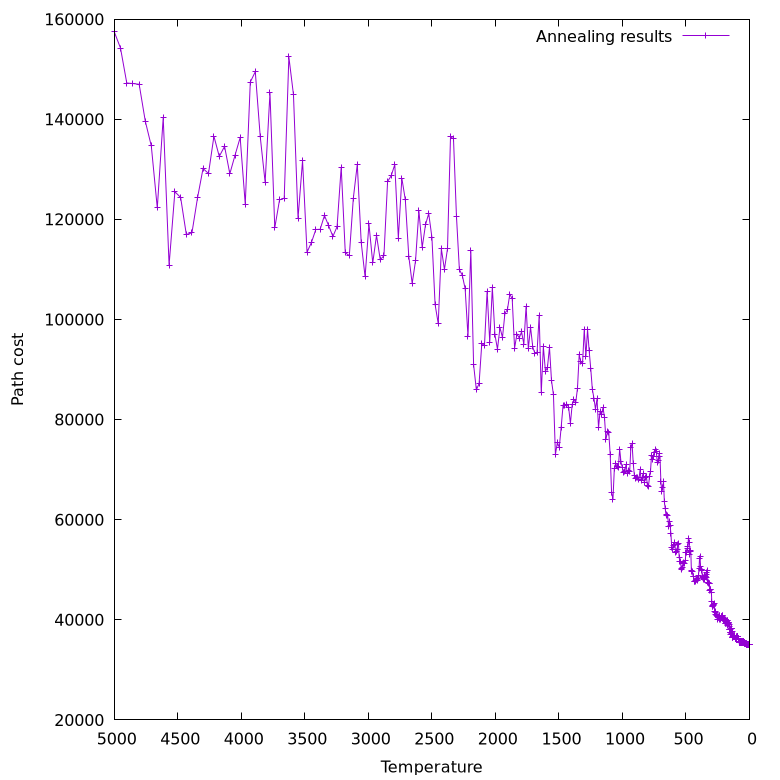
\includegraphics[width=\textwidth]{img/att48.png}
        \caption{The plot showing temperature and cost progression during the simulated annealing process.}
    \end{subfigure}
    \begin{subfigure}[b]{0.49\textwidth}
        \centering
        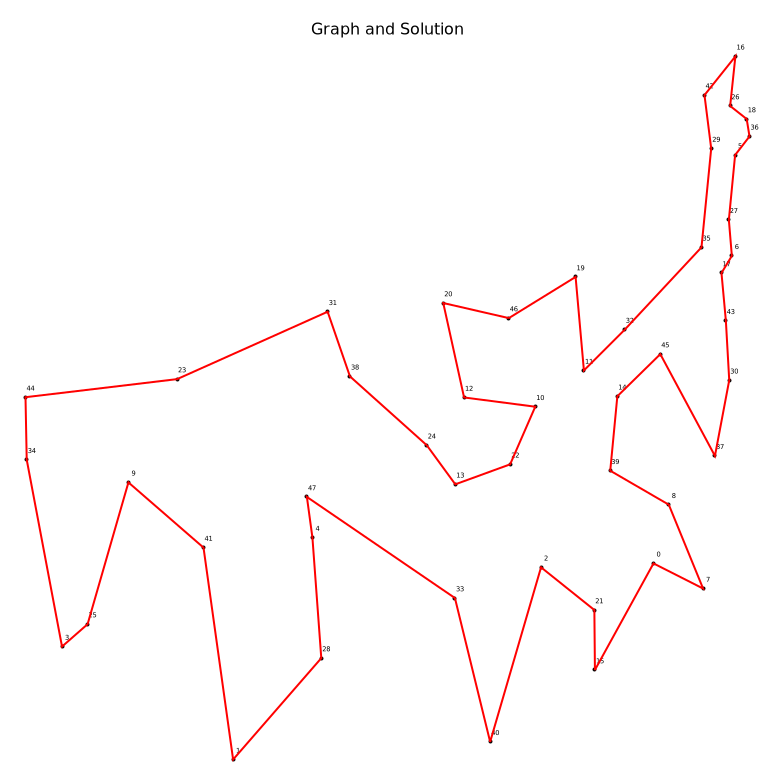
\includegraphics[width=\textwidth]{img/att48_path.png}
        \caption{The plot of the resulting path found by simulated annealing.}
    \end{subfigure}
    \caption{ATT48 Results}
    \label{att48}
\end{figure}

The steps that simulated annealing performed can be obtained by running \textbf{tasp} with the \textit{plot} and \textit{path\_vis} action flags. The generated figures are shown in figure \ref{att48}. The cost does indeed decrease non deterministically and it jumps from one location with local minima to other until eventually reaching the final locally optimal solution at the desired temperature. 

\section{Improvements} \label{impr}

This project had been developed in a time where we had a lot of deadlines and other projects. Therefore, \textbf{tasp} was developed quickly and with the \textit{just-enough} mentality. Therefore, not all the desired functionality had been developed. The todo-list can be viewed on the README page of the GitHub of the project \cite{github}. The highlighted possible improvements are listed here:
\begin{list}{--}{}
    \item Utilize any decreasing temperature function $f: \mathbb{R} \rightarrow \mathbb{R}$ to decrease the temperature instead of hard-coding it.
    \item Create an action that will find the best parameters of the algorithm by itself.
    \item Implement the minimum spanning tree algorithm to provide the lower bound for the TSP, which is very useful in determining whether the algorithm reaches a reasonable optimum.
    \item Use parallel computing to make the algorithm run faster.
\end{list}

\section{Conclusion}

Concluding, even though TSP is a problem that can be solved using a non-deterministic algorithm in the reasonable time, the found results are still very plausible and reasonable to use in real-life world. 

\appendix
\section{Program Code}

The code and installation guide are available on \cite{github}.
\\
\texttt{File execute.c}
\lstinputlisting{src/execute.c}

\texttt{File action\_path.c}
\lstinputlisting{src/action_path.c}

\texttt{File action\_solve.c}
\lstinputlisting{src/action_solve.c}

\texttt{File main.ih}
\lstinputlisting{src/main.ih}

\texttt{File run\_gnuplot.c}
\lstinputlisting{src/run_gnuplot.c}

\texttt{File action\_path\_vis.c}
\lstinputlisting{src/action_path_vis.c}

\texttt{File solve.ih}
\lstinputlisting{src/solve.ih}

\texttt{File sim\_annealing.c}
\lstinputlisting{src/sim_annealing.c}

\texttt{File solve.h}
\lstinputlisting{src/solve.h}

\texttt{File update.c}
\lstinputlisting{src/update.c}

\texttt{File path.h}
\lstinputlisting{src/path.h}

\texttt{File path\_display.c}
\lstinputlisting{src/path_display.c}

\texttt{File path\_shuffle\_invert.c}
\lstinputlisting{src/path_shuffle_invert.c}

\texttt{File path\_shuffle\_display.c}
\lstinputlisting{src/path_shuffle_display.c}

\texttt{File path\_init.c}
\lstinputlisting{src/path_init.c}

\texttt{File path\_compute.c}
\lstinputlisting{src/path_compute.c}

\texttt{File path\_shuffle\_shift.c}
\lstinputlisting{src/path_shuffle_shift.c}

\texttt{File path\_shuffle\_swap.c}
\lstinputlisting{src/path_shuffle_swap.c}

\texttt{File swap.c}
\lstinputlisting{src/swap.c}

\texttt{File path\_shuffle.c}
\lstinputlisting{src/path_shuffle.c}

\texttt{File path\_copy.c}
\lstinputlisting{src/path_copy.c}

\texttt{File path.ih}
\lstinputlisting{src/path.ih}

\texttt{File get\_random\_pair.c}
\lstinputlisting{src/get_random_pair.c}

\texttt{File usage.c}
\lstinputlisting{src/usage.c}

\texttt{File main.c}
\lstinputlisting{src/main.c}

\texttt{File action\_graph.c}
\lstinputlisting{src/action_graph.c}

\texttt{File action\_plot.c}
\lstinputlisting{src/action_plot.c}

\texttt{File parse\_arguments.c}
\lstinputlisting{src/parse_arguments.c}

\texttt{File action\_distances.c}
\lstinputlisting{src/action_distances.c}

\texttt{File action\_graph\_vis.c}
\lstinputlisting{src/action_graph_vis.c}

\texttt{File graph\_create.c}
\lstinputlisting{src/graph_create.c}

\texttt{File action\_graph\_vis\_nol.c}
\lstinputlisting{src/action_graph_vis_nol.c}

\texttt{File graph.ih}
\lstinputlisting{src/graph.ih}

\texttt{File graph\_create\_rand.c}
\lstinputlisting{src/graph_create_rand.c}

\texttt{File graph\_create\_stdin.c}
\lstinputlisting{src/graph_create_stdin.c}

\texttt{File graph\_display.c}
\lstinputlisting{src/graph_display.c}

\texttt{File graph\_distances\_display.c}
\lstinputlisting{src/graph_distances_display.c}

\texttt{File precompute\_distances.c}
\lstinputlisting{src/precompute_distances.c}

\texttt{File graph.h}
\lstinputlisting{src/graph.h}

\texttt{File graph.destroy.c}
\lstinputlisting{src/graph.destroy.c}


\begin{thebibliography}{9}
\bibitem{github}
Artur Topal (2025) TASP, \url{https://github.com/horki-at/tasp}
\end{thebibliography}
\end{document}

